\documentclass{article}
\usepackage[left=2.50cm,right=2.50cm,top=2.50cm,bottom=2.50cm]{geometry}
\usepackage[pdftex]{graphicx}
\usepackage{amsmath, amssymb, }
\usepackage{float}
\usepackage{program}
\usepackage[all]{xy}

\begin{document}

\title{Solution to Homework-2}
\author{Sanath Kumar Ramesh, A50054305}
\date{13-April-2011}
\maketitle

\section{Problem-1}
The solution to this problem follows from Last First Property. According to last first property, the $i^{th}$ occurrence of a character in last column and the $i^{th}$ occurrence of the same character in the first column, correspond to the same character in the original string. Let our original string be represented as $u \epsilon \sigma v$ where $u, v$ are prefix and suffix of the string. $\epsilon,\sigma$ are single characters. \textsc{FindPrev}(B,i) must return $\epsilon$ if $B[i]=\sigma$. By last first property, if $B[i]$ is the $p^{th}$ occurrence of $\sigma$ in the last column, then the last character in the row that has the $p^{th}$ occurrence $\sigma$ in the first column gives $\epsilon$.

\begin{program}
\mbox{\textsc{FindPrev}(B[], Pos[], Occ[], i)}
|Output: previous character|
\BEGIN
	\sigma = B[i]
	p = Occ[\sigma,i]
	rowNum = Pos[\sigma] + p
	|return | B[rowNum]
\END
\end{program}


\noindent \textbf{Example:}
Let the original string be $S = agtct$. Let $\epsilon=|t|$ and $\sigma=|c|$. Therefore, $u=|ag|$ and $v=|t|$. In computing the BW transform, we rotate the string circularly as shown in Table \ref{tab:1}. $\epsilon$ is represented by a bold letter and $\sigma$ by a circled letter. Table \ref{tab:2} shows the strings after sorting them. 

	For $i=5$, $B[5]=c$. $c$ is the 1st occurrence in B[i]. The first occurrence of $c$ in first column happens at row 3. Therefore the last character in row-3 ie. $B[3]$ gives our result. $B[3]=t$, therefore \textbf{t} is our result.

\begin{table}[ht]
	\begin{minipage}[b]{0.4\linewidth}\centering
		\caption{Circularly rotated string}
		\label{tab:1}
		\begin{tabular}{llllll}
			\$ & a & g & \textbf{t} & \textcircled{c} & t \\
			t & \$ & a & g & \textbf{t} & \textcircled{c} \\
			\textcircled{c} & t & \$ & a & g & \textbf{t} \\
			\textbf{t} & \textcircled{c} & t & \$ & a & g \\
			g & \textbf{t} & \textcircled{c} & t & \$ & a \\
			a & g & \textbf{t} & \textcircled{c} & t & \$  \\
		\end{tabular}
	\end{minipage}
	\hspace{0.3cm}
	\begin{minipage}[b]{0.4\linewidth} \centering
		\caption{Sorted Suffix Strings}
		\label{tab:2}
		\begin{tabular}{llllll}
			\$ & a & g & \textbf{t} & \textcircled{c} & t \\
			a & g & \textbf{t} & \textcircled{c} & t & \$  \\
			\textcircled{c} & t & \$ & a & g & \textbf{t} \\
			g & \textbf{t} & \textcircled{c} & t & \$ & a \\									
			t & \$ & a & g & \textbf{t} & \textcircled{c} \\
			\textbf{t} & \textcircled{c} & t & \$ & a & g \\
		\end{tabular}
	\end{minipage}
\end{table}

This algorithm takes constant time to find the previous character and constant extra space.
\section{Problem-2}
The solution to this problem follows from the property of how the original string was rotated. After constructing the BW transform, in any row of the transform, the first character and the last character in that row are always next to each other in the original string. Since the strings have been sorted in ascending order, given the last column ie. B[i], one can compute the first column of the transform. With the first column and last column, one can computer the pairwise ordering of characters in the string. These pairwise orderings can be combined to get back the original string. The procedure is explained with an example: Let the original string be $btatc$. Table \ref{tab:3} gives the cirularly rotated string and Table \ref{tab:4} gives the sorted suffix strings.

\begin{table}[ht]
	\begin{minipage}[b]{0.4\linewidth}\centering
		\caption{Circularly rotated string}
		\label{tab:3}
		\begin{tabular}{llllll}
			\$ & b & t & a & t & c \\
			c & \$ & b & t & a & t \\
			t & c & \$ & b & t & a \\
			a & t & c & \$ & b & t \\
			t & a & t & c & \$ & b \\
			b & t & a & t & c & \$ \\
		\end{tabular}
	\end{minipage}
	\hspace{0.3cm}
	\begin{minipage}[b]{0.4\linewidth} \centering
		\caption{Sorted Suffix Strings}
		\label{tab:4}
		\begin{tabular}{llllll}
			\$ & b & t & a & t & c \\
			a & t & c & \$ & b & t \\
			b & t & a & t & c & \$ \\			
			c & \$ & b & t & a & t \\
			t & a & t & c & \$ & b \\
			t & c & \$ & b & t & a \\
		\end{tabular}
	\end{minipage}
\end{table}

The last column of this transform is given to us as $B[i]$ which is:
\begin{tabular}[l] 
c \\
t \\
\$ \\
t \\
b \\
a \\
\end{tabular}

The algorithm will go through the array $B[i]$ and find the number of occurrences of $\$,a,c,g,t$. In this example, $\$=1,a=1,b=1,c=1,t=2$. This count of the number of occurrences is the first column which we represent by the $count[]$ array.
For this example, $count[0]=1, count[1]=1, count[2]=1, count[3]=1, count[4]=2$. We duplicate this array and name them as $countFirst$ and $countLast$ holding the counts for first column and $B[i]$ which is the last column in the transform.

Now go about constructing the pairwise ordering using $B[i]$ and first column which we have it in the form of $countFirst$. The first column is created by scanning through each each element in the $columnFirst$ array and creating as many alphabets as the count in that position. For above example, we'll create one \$, one $a$, one $b$, one $c$ and two $t$ in order.

For the example, the last column along with the first column is \\

\begin{tabular}{c|c}  
Last column & 1st column \\ \hline
c & \$ \\
t & a \\
\$ & b \\
t & c \\
b & t \\
a & t \\
\end{tabular}

The pairwise ordering is that for some row $i$, the character in the $last\_column[i]$ precedes the character in the $first\_column[i]$ in the original string. With a set of pairwise orderings, to construct the original string one needs to guarantee that all the elements in the ordering are unique. Since here we can have repeating characters, we make them unique by attaching an index along with character. This index is the equal to the occurrence of that character in that column when scanning the column from bottom-up. This index is assigned using the count arrays $countLast$ and $countFirst$. $countLast$ keeps track of the indices for last column and $countFirst$ keeps track of the indices for the first column. For the example, the indices are as follows:

\begin{tabular}{c|c|c|c}  
countLast             & Last column       & 1st column     & countFirst			 \\ \hline
\$=1, a=1, b=1, c=1, t=2 & c$_{1}$           & \$$_{1}$       &  \$=1, a=1, b=1, c=1, t=2\\
\$=1, a=1, b=1, c=0, t=2 & t$_{2}$           & a$_{1}$        &  \$=0, a=1, b=1, c=1, t=2\\
\$=1, a=1, b=1, c=0, t=1 & \$$_{1}$           & b$_{1}$        &  \$=0, a=0 ,b=1 ,c=1, t=2\\
\$=0, a=1, b=1, c=0, t=1 & t$_{1}$           & c$_{1}$        &  \$=0, a=0, b=0, c=1, t=2\\
\$=0, a=1, b=1, c=0, t=0 & b$_{1}$           & t$_{2}$        &  \$=0, a=0, b=0, c=0, t=2\\
\$=0, a=1, b=0, c=0, t=0 & a$_{1}$           & t$_{1}$        &  \$=0, a=0, b=0, c=0, t=1\\
\$=0, a=0, b=0, c=0, t=0 &                   &                &  \$=0, a=0, b=0, c=0, t=0\\
\end{tabular}

Now the pairwise ordering is as follows:
\begin{displaymath}
  \xymatrix{ 
 c_{1}  \ar[r] & \$_{1} \\
 t_{2}  \ar[r] & a_{1} \\
 \$_{1} \ar[r] & b_{1}\\
 t_{1}  \ar[r] & c_{1} \\
 b_{1} \ar[r]  & t_{2} \\
a_{1}   \ar[r] & t_{1}  \\ }
\end{displaymath}

Now join the orderings using transitive relationship. This will yield the following complete ordering. 

\begin{displaymath}
  \xymatrix{ 
   \$_{1} \ar[r] & b_{1} \ar[r]  & t_{2} \ar[r] & a_{1} \ar[r] & t_{1} \ar[r] & c_{1} \\
 }
\end{displaymath}

Dropping the indices and \$ gives the original string - $btatc$.

\begin{program}
\mbox{Algorithm construct-string(B)}
|Output: original string|
\BEGIN
	countFirst[\ ] = countLast[\ ] = findCounts(B)
	ordering = \{\}
	first\_col\_ptr=1 \rcomment{// Tracks the non-zero count character countFirst}
	\FOR i in B \DO
		x = character\_at(first\_col\_ptr)
		y = B[i]
		X = < \ x,\ countFirst[first\_col\_ptr] \ >
		Y = < \ y,\ count\_at(countLast, y)) \ >
		ordering = ordering \union {X,Y}
		
		countFirst[first\_col\_ptr] = countFirst[first\_col\_ptr] - 1
		\IF countFirst[first\_col\_ptr] == 0 | then |
			first\_col\_ptr = first\_col\_ptr + 1
		\FI

		decrement\_count(countLast, y)
	\OD
	
\END
\end{program}

\begin{program}
\mbox{function character\_at(pos)}
|Output: character denoted by pos |
\BEGIN
	\IF pos == 0 | then return '\$'|
	\ELSE | if | pos == 1 | then return 'a'|
	\ELSE | if | pos == 2 | then return  'c'|
	\ELSE | if | pos == 3 | then return  'g'|
	\ELSE |  return  't'|
	\FI
\END
\end{program}


\begin{program}
\mbox{function decrement\_count(countArray, char)}
|Output: none |
\BEGIN
	\IF char == |'\$' then |countArray[0] = countArray[0] - 1 
	|else if | char == |'a' then |countArray[1] = countArray[1] -1 
	|else if | char == |'c' then |countArray[2] = countArray[2] -1 
	|else if | char == |'g' then |countArray[3] = countArray[3] -1
	|else | countArray[4]= countArray[4] -1 
	\FI
\END
\end{program}

\begin{program}
\mbox{function count\_at(countArray, char)}
|Output: value of countArray corresponding to char |
\BEGIN
	\IF char == |'\$' then return | countArray[0]
	|else if | char == |'a' then return |countArray[1]
	|else if | char == |'c' then return |countArray[2]
	|else if | char == |'g' then return |countArray[3]
	|else return | countArray[4]
	\FI
\END
\end{program}

\section{Problem-3}
This may not be a good idea for compression because, BW transform of a string is going to be very different from the original string. In case the original string had many recurring patterns, then BW transformed string might break those patterns making it less amenable to compression. 

\section{Problem-4}
The pseudo-code for my program is as follows:
\begin{program}
\mbox{Algorithm FindRepeat(DNA)}
\BEGIN
	KeywordTree=\{\}
	OutputList=\{\}
	
	\FOR | each substring | s | of length 16 from DNA| \DO
		pos = | position of beginning of | s
		posList = Add(KeywordTree,s, pos)
		\IF OutputList.exists(posList) == false | then |
			OutputList.add(posList) 
			\ \rcomment{/* posList is added as a reference to OutputList }
			\ \rcomment{Changes made on the posList through KeywordTree will reflect here */} 
		\FI
	\OD
	|print | OutputList
\END	
\end{program}

\begin{program}
\mbox{function Add(KeywordTree, s, pos)}
\BEGIN
	current\_node = KeywordTree.root
	\FOR i = 1 to 16 \DO
		\IF current\_node[\ s[i]\ ] == NULL | then |
			node = create_new_node()
			current\_node[\ s[i]\ ] = node
		\FI
		current\_node = current\_node[\ s[i]\ ] 
	\OD
	\COMMENT{Last node in KeywordTree will have pointer to position-list}
	\IF current\_node.posListExists == false | then | 
		posList = create_pos_list()
		posList = (s, pos)
		current\_node.postList = posList
		|return | posList
	\ELSE
		posList = current\_node.posList
		posList.add(pos)
		|return | posList
	\FI	
\END
\end{program}

Explaining in words, split DNA sequence into substrings of 16characters. Using these strings, construct a Keyword Tree. The leaf node of the keyword tree will point to a list called position-list. This list stores the starting position of substring in DNA sequence. When another occurrence of the same string is encountered, an existing path will be traversed by the algorithm to reach the final node. In the position-list attached to the final node, add the starting position of this string. Thus, position-list at each leaf node will have a list of starting positions of the substring in DNA sequence. To make the algorithm faster, another list called OutputList keeps record of the position-lists attached to the leaf nodes. Thus after the whole DNA sequence has been traversed, the OutputList will hold the position-list corresponding to each and every substring in the DNA. In a KeywordTree, since each substring has a unique path from root to the leaf node, the repetition counts of all substrings in the DNA can be found in just one traversal of the DNA sequence. Thus this algorithm has $O(n)$ time and $O(n)$ space complexity.

\subsection{Expected number of repeats}
	Since each base is equally likely, each has a probability of $1/4$. For a DNA sequence, each letter in the sequence has 4 possibilities. For a sequence of length $16$, there are $4^{16}$ possible combinations of bases. For DNA sequence of length $N$, there are $N-15$ substrings of length 16. For large $N$, $N-15 \approx N$. Therefor, there are $N$ different substrings of length 16 possible from a DNA sequence of length $N$.

	Since there are $4^{16}$ possible substrings of length 16, the probability of getting one particular substring is $1/4^{16}$. Probability of finding two same substrings then becomes $(1/4^{16}) * (1/4^{16})$. Modeling this process as a Binomial Distribution, the expected number of repeats with N substrings is $N*(1/4^{16}) * (1/4^{16})$

	For $N = 4^{12}$, the expected value is $1/4^{20}$!! This number is really small. It is clearly shown by the number of repeats observed. This is shown in Figure \ref{histogram}. The raw data provides more clear picture of the trend. It is shown in Table \ref{tab:hist}. \\

\begin{table}
\caption{Frequency of repeats seen}
\label{tab:hist}	
\begin{tabular}{|c|c|c|c|}
\hline
	&	1 repeats	& 2 repeats	& 3 repeats \\ \hline
$4^{7}$	& 163690 &	0	& 0 \\ \hline
$4^8$	& 655202	& 4	& 0 \\ \hline
$4^9$	& 2621170 &	60 &	0 \\ \hline
$4^{10}$	& 10483110 & 	1250 &	0 \\ \hline
$4^{11}$ & 	41902166 &	20359	& 2 \\ \hline
\end{tabular}
\end{table}

\begin{figure}
		\centering
		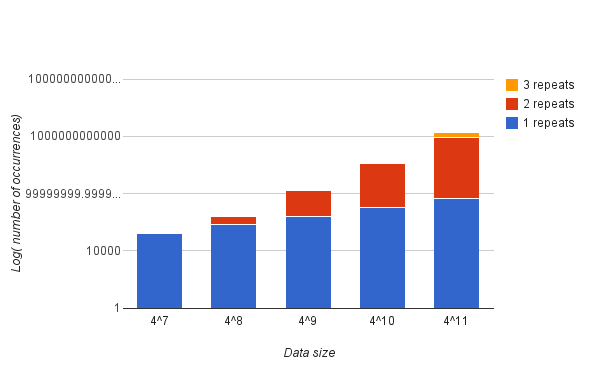
\includegraphics[scale=0.5]{chart_1.png}
				\caption{Number of occurrences of repeats in log scale. I was unable to get data for $4^{12}$ size}
		\label{histogram}

\end{figure}

\begin{figure}
		\centering
		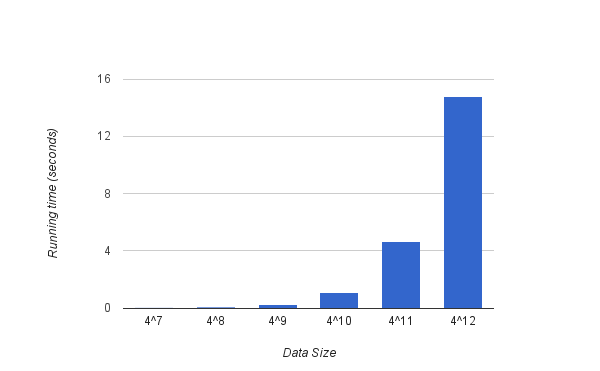
\includegraphics[scale=0.6]{chart_2.png}
		\caption{Running time of code on various data sizes}
		\label{runtime}
		
\end{figure}	
Such dramatically low number for 2-repeats and 3-repeats is because of the low probablity of finding one substring as described above.


The Figure \ref{runtime} shows the running time as a function of data size. The algorithm scales really well with data size. This is because along with the data structure construction, the algorithm finds the position of repeats.
\end{document}

